The DEF compiler is based on the Tapir branch of LLVM, that provides fork-join parallelism primitives.\cite{TAPIR}\cite{LLVM}  The front-end is principly written in OCaml.  Likewise, the \texttt{defghi} utility is written in OCaml.\cite{DEF}

\subsection{Basic Syntax}

\begin{figure}[htbp!]
        \centering
        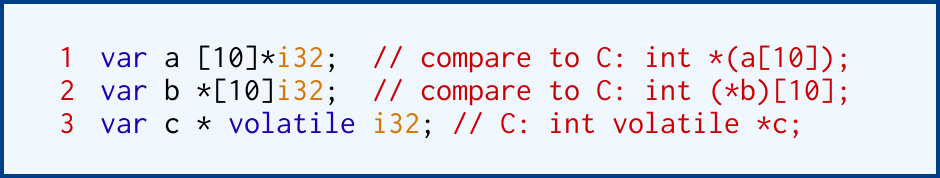
\includegraphics[scale=0.25]{gfx/types}
        \caption{Examples of variable declarations in DEF.  C allows the parentheses to be omitted in the first case, though they're provided to make precedence explicit.}
        \label{fig:types}
\end{figure}

Syntactically, DEF looks similar to C with the most apparent difference being that scopes are denoted by keywords instead of curly braces and curly braces are used for tuples.  Native types specify a bit width, so C's \texttt{int} on most systems corresponds to DEF's \texttt{i32}.  Types are also designed to read left-to-right, so the return type in a function declaration has been moved to the right using an arrow notation similar to ML-like languages or Go.  For more complicated types, fig.~\ref{fig:types} gives an example of left-to-rightness where no parentheses are needed to distinguish an array of pointers to integers (line 1) from a pointer to an array of 32-bit integers (line 2).

\begin{figure}[htbp!]
        \centering
        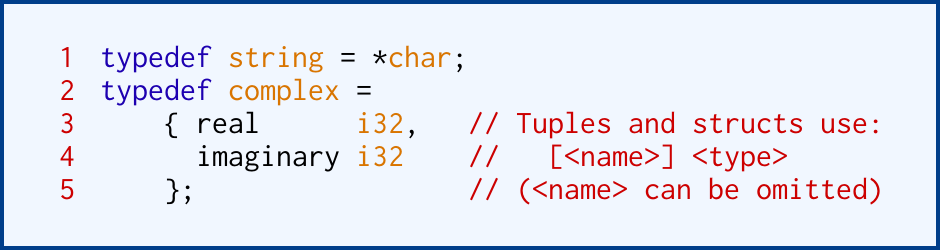
\includegraphics[scale=0.25]{gfx/typedef}
        \caption{Defining types with \texttt{typedef}.}
        \label{fig:typedef}
\end{figure}

Types are defined with the \texttt{typedef} keyword.  Figure \ref{fig:typedef} shows two examples: a C-style \texttt{string} type is defined on line 1, and a complex number struct is defined on lines 2-5.
